\documentclass[]{article}
\usepackage{lmodern}
\usepackage{amssymb,amsmath}
\usepackage{ifxetex,ifluatex}
\usepackage{fixltx2e} % provides \textsubscript
\ifnum 0\ifxetex 1\fi\ifluatex 1\fi=0 % if pdftex
  \usepackage[T1]{fontenc}
  \usepackage[utf8]{inputenc}
\else % if luatex or xelatex
  \ifxetex
    \usepackage{mathspec}
  \else
    \usepackage{fontspec}
  \fi
  \defaultfontfeatures{Ligatures=TeX,Scale=MatchLowercase}
\fi
% use upquote if available, for straight quotes in verbatim environments
\IfFileExists{upquote.sty}{\usepackage{upquote}}{}
% use microtype if available
\IfFileExists{microtype.sty}{%
\usepackage{microtype}
\UseMicrotypeSet[protrusion]{basicmath} % disable protrusion for tt fonts
}{}
\usepackage[margin=1in]{geometry}
\usepackage{hyperref}
\hypersetup{unicode=true,
            pdftitle={What Makes the Best Tennis Player?},
            pdfauthor={Steven Herrera and Ethan Shen},
            pdfborder={0 0 0},
            breaklinks=true}
\urlstyle{same}  % don't use monospace font for urls
\usepackage{color}
\usepackage{fancyvrb}
\newcommand{\VerbBar}{|}
\newcommand{\VERB}{\Verb[commandchars=\\\{\}]}
\DefineVerbatimEnvironment{Highlighting}{Verbatim}{commandchars=\\\{\}}
% Add ',fontsize=\small' for more characters per line
\usepackage{framed}
\definecolor{shadecolor}{RGB}{248,248,248}
\newenvironment{Shaded}{\begin{snugshade}}{\end{snugshade}}
\newcommand{\AlertTok}[1]{\textcolor[rgb]{0.94,0.16,0.16}{#1}}
\newcommand{\AnnotationTok}[1]{\textcolor[rgb]{0.56,0.35,0.01}{\textbf{\textit{#1}}}}
\newcommand{\AttributeTok}[1]{\textcolor[rgb]{0.77,0.63,0.00}{#1}}
\newcommand{\BaseNTok}[1]{\textcolor[rgb]{0.00,0.00,0.81}{#1}}
\newcommand{\BuiltInTok}[1]{#1}
\newcommand{\CharTok}[1]{\textcolor[rgb]{0.31,0.60,0.02}{#1}}
\newcommand{\CommentTok}[1]{\textcolor[rgb]{0.56,0.35,0.01}{\textit{#1}}}
\newcommand{\CommentVarTok}[1]{\textcolor[rgb]{0.56,0.35,0.01}{\textbf{\textit{#1}}}}
\newcommand{\ConstantTok}[1]{\textcolor[rgb]{0.00,0.00,0.00}{#1}}
\newcommand{\ControlFlowTok}[1]{\textcolor[rgb]{0.13,0.29,0.53}{\textbf{#1}}}
\newcommand{\DataTypeTok}[1]{\textcolor[rgb]{0.13,0.29,0.53}{#1}}
\newcommand{\DecValTok}[1]{\textcolor[rgb]{0.00,0.00,0.81}{#1}}
\newcommand{\DocumentationTok}[1]{\textcolor[rgb]{0.56,0.35,0.01}{\textbf{\textit{#1}}}}
\newcommand{\ErrorTok}[1]{\textcolor[rgb]{0.64,0.00,0.00}{\textbf{#1}}}
\newcommand{\ExtensionTok}[1]{#1}
\newcommand{\FloatTok}[1]{\textcolor[rgb]{0.00,0.00,0.81}{#1}}
\newcommand{\FunctionTok}[1]{\textcolor[rgb]{0.00,0.00,0.00}{#1}}
\newcommand{\ImportTok}[1]{#1}
\newcommand{\InformationTok}[1]{\textcolor[rgb]{0.56,0.35,0.01}{\textbf{\textit{#1}}}}
\newcommand{\KeywordTok}[1]{\textcolor[rgb]{0.13,0.29,0.53}{\textbf{#1}}}
\newcommand{\NormalTok}[1]{#1}
\newcommand{\OperatorTok}[1]{\textcolor[rgb]{0.81,0.36,0.00}{\textbf{#1}}}
\newcommand{\OtherTok}[1]{\textcolor[rgb]{0.56,0.35,0.01}{#1}}
\newcommand{\PreprocessorTok}[1]{\textcolor[rgb]{0.56,0.35,0.01}{\textit{#1}}}
\newcommand{\RegionMarkerTok}[1]{#1}
\newcommand{\SpecialCharTok}[1]{\textcolor[rgb]{0.00,0.00,0.00}{#1}}
\newcommand{\SpecialStringTok}[1]{\textcolor[rgb]{0.31,0.60,0.02}{#1}}
\newcommand{\StringTok}[1]{\textcolor[rgb]{0.31,0.60,0.02}{#1}}
\newcommand{\VariableTok}[1]{\textcolor[rgb]{0.00,0.00,0.00}{#1}}
\newcommand{\VerbatimStringTok}[1]{\textcolor[rgb]{0.31,0.60,0.02}{#1}}
\newcommand{\WarningTok}[1]{\textcolor[rgb]{0.56,0.35,0.01}{\textbf{\textit{#1}}}}
\usepackage{longtable,booktabs}
\usepackage{graphicx,grffile}
\makeatletter
\def\maxwidth{\ifdim\Gin@nat@width>\linewidth\linewidth\else\Gin@nat@width\fi}
\def\maxheight{\ifdim\Gin@nat@height>\textheight\textheight\else\Gin@nat@height\fi}
\makeatother
% Scale images if necessary, so that they will not overflow the page
% margins by default, and it is still possible to overwrite the defaults
% using explicit options in \includegraphics[width, height, ...]{}
\setkeys{Gin}{width=\maxwidth,height=\maxheight,keepaspectratio}
\IfFileExists{parskip.sty}{%
\usepackage{parskip}
}{% else
\setlength{\parindent}{0pt}
\setlength{\parskip}{6pt plus 2pt minus 1pt}
}
\setlength{\emergencystretch}{3em}  % prevent overfull lines
\providecommand{\tightlist}{%
  \setlength{\itemsep}{0pt}\setlength{\parskip}{0pt}}
\setcounter{secnumdepth}{0}
% Redefines (sub)paragraphs to behave more like sections
\ifx\paragraph\undefined\else
\let\oldparagraph\paragraph
\renewcommand{\paragraph}[1]{\oldparagraph{#1}\mbox{}}
\fi
\ifx\subparagraph\undefined\else
\let\oldsubparagraph\subparagraph
\renewcommand{\subparagraph}[1]{\oldsubparagraph{#1}\mbox{}}
\fi

%%% Use protect on footnotes to avoid problems with footnotes in titles
\let\rmarkdownfootnote\footnote%
\def\footnote{\protect\rmarkdownfootnote}

%%% Change title format to be more compact
\usepackage{titling}

% Create subtitle command for use in maketitle
\newcommand{\subtitle}[1]{
  \posttitle{
    \begin{center}\large#1\end{center}
    }
}

\setlength{\droptitle}{-2em}

  \title{What Makes the Best Tennis Player?}
    \pretitle{\vspace{\droptitle}\centering\huge}
  \posttitle{\par}
    \author{Steven Herrera and Ethan Shen}
    \preauthor{\centering\large\emph}
  \postauthor{\par}
      \predate{\centering\large\emph}
  \postdate{\par}
    \date{11/09/2018}


\begin{document}
\maketitle

\hypertarget{loaded-packages}{%
\section{Loaded Packages}\label{loaded-packages}}

\begin{Shaded}
\begin{Highlighting}[]
\KeywordTok{library}\NormalTok{(tidyverse)}
\KeywordTok{library}\NormalTok{(olsrr)}
\KeywordTok{library}\NormalTok{(cowplot)}
\KeywordTok{library}\NormalTok{(car)}
\KeywordTok{library}\NormalTok{(broom)}
\KeywordTok{library}\NormalTok{(knitr)}
\KeywordTok{library}\NormalTok{(arm)}
\KeywordTok{library}\NormalTok{(tidyr)}
\KeywordTok{library}\NormalTok{(pROC)}
\KeywordTok{library}\NormalTok{(arm)}
\KeywordTok{library}\NormalTok{(rlm)}
\end{Highlighting}
\end{Shaded}

\hypertarget{data-manipulation}{%
\section{Data Manipulation}\label{data-manipulation}}

\begin{Shaded}
\begin{Highlighting}[]
\NormalTok{atp <-}\StringTok{ }\KeywordTok{read_csv}\NormalTok{(}\StringTok{"files/atp.csv"}\NormalTok{)}
\NormalTok{atp2016 <-}\StringTok{ }\KeywordTok{read_csv}\NormalTok{(}\StringTok{"files/atp2016.csv"}\NormalTok{)}
\NormalTok{atp2015 <-}\StringTok{ }\KeywordTok{read_csv}\NormalTok{(}\StringTok{"files/atp2015.csv"}\NormalTok{)}
\NormalTok{atp2014 <-}\StringTok{ }\KeywordTok{read_csv}\NormalTok{(}\StringTok{"files/atp2014.csv"}\NormalTok{)}
\NormalTok{atp2013 <-}\StringTok{ }\KeywordTok{read_csv}\NormalTok{(}\StringTok{"files/atp2013.csv"}\NormalTok{)}
\NormalTok{atp2012 <-}\StringTok{ }\KeywordTok{read_csv}\NormalTok{(}\StringTok{"files/atp2012.csv"}\NormalTok{)}
\NormalTok{atp2011 <-}\StringTok{ }\KeywordTok{read_csv}\NormalTok{(}\StringTok{"files/atp2011.csv"}\NormalTok{)}
\NormalTok{atp2010 <-}\StringTok{ }\KeywordTok{read_csv}\NormalTok{(}\StringTok{"files/atp2010.csv"}\NormalTok{)}

\NormalTok{atp1 <-}\StringTok{ }\NormalTok{atp }\OperatorTok
\StringTok{  }\KeywordTok{filter}\NormalTok{(tourney_date }\OperatorTok{<}\StringTok{ }\DecValTok{20171113}\NormalTok{)}

\NormalTok{winners2016 <-}\StringTok{ }\NormalTok{atp2016 }\OperatorTok
\StringTok{  }\KeywordTok{filter}\NormalTok{(tourney_date }\OperatorTok{<}\StringTok{ }\DecValTok{20161114}\NormalTok{)}

\NormalTok{winners2015 <-}\StringTok{ }\NormalTok{atp2015 }\OperatorTok
\StringTok{  }\KeywordTok{filter}\NormalTok{(tourney_date }\OperatorTok{<}\StringTok{ }\DecValTok{20151115}\NormalTok{) }

\NormalTok{winners2014 <-}\StringTok{ }\NormalTok{atp2014 }\OperatorTok
\StringTok{  }\KeywordTok{filter}\NormalTok{(tourney_date }\OperatorTok{<}\StringTok{ }\DecValTok{20141109}\NormalTok{) }

\NormalTok{winners2013 <-}\StringTok{ }\NormalTok{atp2013 }\OperatorTok
\StringTok{  }\KeywordTok{filter}\NormalTok{(tourney_date }\OperatorTok{<}\StringTok{ }\DecValTok{20131104}\NormalTok{) }

\NormalTok{winners2012 <-}\StringTok{ }\NormalTok{atp2012 }\OperatorTok
\StringTok{  }\KeywordTok{filter}\NormalTok{(tourney_date }\OperatorTok{<}\StringTok{ }\DecValTok{20121105}\NormalTok{) }

\NormalTok{winners2011 <-}\StringTok{ }\NormalTok{atp2011 }\OperatorTok
\StringTok{  }\KeywordTok{filter}\NormalTok{(tourney_date }\OperatorTok{<}\StringTok{ }\DecValTok{20111114}\NormalTok{) }

\NormalTok{winners2010 <-}\StringTok{ }\NormalTok{atp2010 }\OperatorTok
\StringTok{  }\KeywordTok{filter}\NormalTok{(tourney_date }\OperatorTok{<}\StringTok{ }\DecValTok{20101121}\NormalTok{) }

\NormalTok{winners <-}\StringTok{ }\KeywordTok{rbind}\NormalTok{(atp1, winners2016, winners2015, winners2014, winners2013, }
\NormalTok{                 winners2012, winners2011, winners2010)}

\NormalTok{winners_set <-}\StringTok{ }\NormalTok{winners }\OperatorTok
\StringTok{  }\KeywordTok{filter}\NormalTok{(best_of }\OperatorTok{==}\StringTok{ }\DecValTok{3}\NormalTok{,}
         \OperatorTok{!}\KeywordTok{is.na}\NormalTok{(w_ace), }
         \OperatorTok{!}\KeywordTok{is.na}\NormalTok{(w_df), }
         \OperatorTok{!}\KeywordTok{is.na}\NormalTok{(w_svpt), }
         \OperatorTok{!}\KeywordTok{is.na}\NormalTok{(w_1stIn), }
         \OperatorTok{!}\KeywordTok{is.na}\NormalTok{(w_1stWon), }
         \OperatorTok{!}\KeywordTok{is.na}\NormalTok{(w_2ndWon),}
         \OperatorTok{!}\KeywordTok{is.na}\NormalTok{(w_SvGms), }
         \OperatorTok{!}\KeywordTok{is.na}\NormalTok{(w_bpSaved),}
         \OperatorTok{!}\KeywordTok{is.na}\NormalTok{(w_bpFaced),}
\NormalTok{         surface}\OperatorTok{!=}\StringTok{"None"}\NormalTok{)}

\NormalTok{losers <-}\StringTok{ }\NormalTok{winners_set }\OperatorTok
\StringTok{  }\KeywordTok{mutate}\NormalTok{(}\DataTypeTok{seed =}\NormalTok{ loser_seed,}
         \DataTypeTok{name =}\NormalTok{ loser_name,}
         \DataTypeTok{hand =}\NormalTok{ loser_hand,}
         \DataTypeTok{ht =}\NormalTok{ loser_ht,}
         \DataTypeTok{age =}\NormalTok{ loser_age,}
         \DataTypeTok{rank =}\NormalTok{ loser_rank,}
         \DataTypeTok{rankpoints =}\NormalTok{ loser_rank_points,}
         \DataTypeTok{ace =}\NormalTok{ l_ace,}
         \DataTypeTok{df =}\NormalTok{ l_df,}
         \DataTypeTok{svpt =}\NormalTok{ l_svpt,}
         \DataTypeTok{firsstIn =}\NormalTok{ l_1stIn,}
         \DataTypeTok{firsttWon =}\NormalTok{ l_1stWon,}
         \DataTypeTok{secondndWon =}\NormalTok{ l_2ndWon,}
         \DataTypeTok{SvGms =}\NormalTok{ l_SvGms,}
         \DataTypeTok{bpSaved =}\NormalTok{ l_bpSaved,}
         \DataTypeTok{bpFaced =}\NormalTok{ l_bpFaced,}
         \DataTypeTok{minutes =}\NormalTok{ minutes,}
         \DataTypeTok{status =} \DecValTok{0}
\NormalTok{         )  }
  

\NormalTok{winners <-}\StringTok{ }\NormalTok{winners_set }\OperatorTok
\StringTok{  }\KeywordTok{mutate}\NormalTok{(}\DataTypeTok{seed =}\NormalTok{ winner_seed,}
         \DataTypeTok{name =}\NormalTok{ winner_name,}
         \DataTypeTok{hand =}\NormalTok{ winner_hand,}
         \DataTypeTok{ht =}\NormalTok{ winner_ht,}
         \DataTypeTok{age =}\NormalTok{ winner_age,}
         \DataTypeTok{rank =}\NormalTok{ winner_rank,}
         \DataTypeTok{rankpoints =}\NormalTok{ winner_rank_points,}
         \DataTypeTok{ace =}\NormalTok{ w_ace,}
         \DataTypeTok{df =}\NormalTok{ w_df,}
         \DataTypeTok{svpt =}\NormalTok{ w_svpt,}
         \DataTypeTok{firsstIn =}\NormalTok{ w_1stIn,}
         \DataTypeTok{firsttWon =}\NormalTok{ w_1stWon,}
         \DataTypeTok{secondndWon =}\NormalTok{ w_2ndWon,}
         \DataTypeTok{SvGms =}\NormalTok{ w_SvGms,}
         \DataTypeTok{bpSaved =}\NormalTok{ w_bpSaved,}
         \DataTypeTok{bpFaced =}\NormalTok{ w_bpFaced,}
         \DataTypeTok{minutes =}\NormalTok{ minutes,}
         \DataTypeTok{status =} \DecValTok{1}
\NormalTok{         ) }
\NormalTok{tennis <-}\StringTok{ }\KeywordTok{rbind}\NormalTok{(winners,losers)}

\NormalTok{tennis <-}\StringTok{ }\NormalTok{tennis }\OperatorTok
\StringTok{  }\KeywordTok{filter}\NormalTok{(}\OperatorTok{!}\KeywordTok{is.na}\NormalTok{(seed),}
         \OperatorTok{!}\KeywordTok{is.na}\NormalTok{(name),}
         \OperatorTok{!}\KeywordTok{is.na}\NormalTok{(hand),}
         \OperatorTok{!}\KeywordTok{is.na}\NormalTok{(ht),}
         \OperatorTok{!}\KeywordTok{is.na}\NormalTok{(age),}
         \OperatorTok{!}\KeywordTok{is.na}\NormalTok{(rank),}
         \OperatorTok{!}\KeywordTok{is.na}\NormalTok{(rankpoints),}
         \OperatorTok{!}\KeywordTok{is.na}\NormalTok{(ace),}
         \OperatorTok{!}\KeywordTok{is.na}\NormalTok{(df),}
         \OperatorTok{!}\KeywordTok{is.na}\NormalTok{(svpt),}
         \OperatorTok{!}\KeywordTok{is.na}\NormalTok{(firsstIn),}
         \OperatorTok{!}\KeywordTok{is.na}\NormalTok{(firsttWon),}
         \OperatorTok{!}\KeywordTok{is.na}\NormalTok{(secondndWon),}
         \OperatorTok{!}\KeywordTok{is.na}\NormalTok{(SvGms),}
         \OperatorTok{!}\KeywordTok{is.na}\NormalTok{(bpSaved),}
         \OperatorTok{!}\KeywordTok{is.na}\NormalTok{(bpFaced),}
         \OperatorTok{!}\KeywordTok{is.na}\NormalTok{(minutes),}
         \OperatorTok{!}\KeywordTok{is.na}\NormalTok{(status))}
\end{Highlighting}
\end{Shaded}

\hypertarget{data}{%
\section{Data}\label{data}}

Using data manipulation skills in R, we shaped the dataset to show each
observation as the outcome of the match for the winner and the loser of
each match from 2010-2017. Below, is a glimpse of our dataset.

\begin{Shaded}
\begin{Highlighting}[]
\KeywordTok{glimpse}\NormalTok{(tennis)}
\end{Highlighting}
\end{Shaded}

\begin{verbatim}
## Observations: 11,037
## Variables: 66
## $ tourney_id         <chr> "2017-M020", "2017-M020", "2017-M020", "201...
## $ tourney_name       <chr> "Brisbane", "Brisbane", "Brisbane", "Brisba...
## $ surface            <chr> "Hard", "Hard", "Hard", "Hard", "Hard", "Ha...
## $ draw_size          <int> 32, 32, 32, 32, 32, 32, 32, 32, 32, 32, 32,...
## $ tourney_level      <chr> "A", "A", "A", "A", "A", "A", "A", "A", "A"...
## $ tourney_date       <int> 20170102, 20170102, 20170102, 20170102, 201...
## $ match_num          <int> 300, 299, 298, 297, 296, 295, 294, 293, 292...
## $ winner_id          <int> 105777, 105777, 105453, 105683, 105777, 105...
## $ winner_seed        <int> 7, 7, 3, 1, 7, 3, 2, 1, 5, 4, 7, 3, 2, 5, 7...
## $ winner_entry       <chr> NA, NA, NA, NA, NA, NA, NA, NA, NA, NA, NA,...
## $ winner_name        <chr> "Grigor Dimitrov", "Grigor Dimitrov", "Kei ...
## $ winner_hand        <chr> "R", "R", "R", "R", "R", "R", "R", "R", "L"...
## $ winner_ht          <int> 188, 188, 178, 196, 188, 178, 183, 196, 185...
## $ winner_ioc         <chr> "BUL", "BUL", "JPN", "CAN", "BUL", "JPN", "...
## $ winner_age         <dbl> 25.63450, 25.63450, 27.01164, 26.01780, 25....
## $ winner_rank        <int> 17, 17, 5, 3, 17, 5, 4, 3, 9, 8, 17, 5, 4, ...
## $ winner_rank_points <int> 2035, 2035, 4905, 5450, 2035, 4905, 5315, 5...
## $ loser_id           <int> 105453, 105683, 104527, 104745, 106233, 111...
## $ loser_seed         <int> 3, 1, 2, 5, 4, NA, NA, NA, NA, NA, NA, NA, ...
## $ loser_entry        <chr> NA, NA, NA, NA, NA, "WC", NA, NA, NA, "WC",...
## $ loser_name         <chr> "Kei Nishikori", "Milos Raonic", "Stanislas...
## $ loser_hand         <chr> "R", "R", "R", "L", "R", "R", "R", "R", "L"...
## $ loser_ht           <int> 178, 196, 183, 185, 185, NA, NA, 170, 190, ...
## $ loser_ioc          <chr> "JPN", "CAN", "SUI", "ESP", "AUT", "AUS", "...
## $ loser_age          <dbl> 27.01164, 26.01780, 31.76728, 30.58453, 23....
## $ loser_rank         <int> 5, 3, 4, 9, 8, 79, 45, 52, 51, 180, 39, 105...
## $ loser_rank_points  <int> 4905, 5450, 5315, 3300, 3415, 689, 1001, 86...
## $ score              <chr> "6-2 2-6 6-3", "7-6(7) 6-2", "7-6(3) 6-3", ...
## $ best_of            <int> 3, 3, 3, 3, 3, 3, 3, 3, 3, 3, 3, 3, 3, 3, 3...
## $ round              <chr> "F", "SF", "SF", "QF", "QF", "QF", "QF", "R...
## $ minutes            <int> 108, 87, 101, 140, 124, 61, 156, 69, 55, 89...
## $ w_ace              <int> 7, 4, 1, 23, 3, 3, 11, 12, 1, 11, 8, 3, 7, ...
## $ w_df               <int> 2, 1, 1, 3, 3, 0, 3, 1, 2, 1, 0, 3, 2, 1, 0...
## $ w_svpt             <int> 77, 58, 77, 97, 94, 34, 119, 53, 38, 65, 46...
## $ w_1stIn            <int> 52, 36, 56, 62, 52, 19, 67, 40, 18, 44, 27,...
## $ w_1stWon           <int> 41, 27, 37, 50, 42, 18, 47, 30, 15, 36, 25,...
## $ w_2ndWon           <int> 12, 18, 14, 16, 23, 10, 28, 7, 15, 15, 12, ...
## $ w_SvGms            <int> 13, 10, 11, 15, 14, 7, 16, 9, 7, 11, 9, 15,...
## $ w_bpSaved          <int> 5, 0, 4, 6, 13, 0, 11, 2, 2, 4, 3, 4, 0, 2,...
## $ w_bpFaced          <int> 7, 0, 5, 7, 14, 0, 13, 3, 2, 4, 3, 8, 1, 3,...
## $ l_ace              <int> 4, 4, 9, 4, 6, 1, 2, 0, 2, 11, 4, 6, 5, 2, ...
## $ l_df               <int> 0, 3, 2, 0, 5, 2, 2, 1, 2, 1, 3, 4, 7, 2, 3...
## $ l_svpt             <int> 69, 61, 61, 84, 82, 47, 97, 44, 38, 58, 52,...
## $ l_1stIn            <int> 49, 28, 37, 61, 37, 28, 65, 29, 25, 35, 37,...
## $ l_1stWon           <int> 36, 24, 27, 39, 29, 15, 52, 17, 13, 34, 27,...
## $ l_2ndWon           <int> 9, 16, 10, 14, 24, 5, 11, 6, 3, 9, 4, 20, 8...
## $ l_SvGms            <int> 12, 10, 10, 14, 14, 7, 16, 8, 7, 10, 9, 14,...
## $ l_bpSaved          <int> 2, 2, 0, 2, 4, 3, 6, 2, 3, 3, 0, 8, 3, 0, 4...
## $ l_bpFaced          <int> 5, 4, 2, 4, 7, 8, 10, 6, 8, 4, 3, 13, 5, 4,...
## $ seed               <int> 7, 7, 3, 1, 7, 3, 2, 1, 5, 4, 7, 3, 2, 5, 7...
## $ name               <chr> "Grigor Dimitrov", "Grigor Dimitrov", "Kei ...
## $ hand               <chr> "R", "R", "R", "R", "R", "R", "R", "R", "L"...
## $ ht                 <int> 188, 188, 178, 196, 188, 178, 183, 196, 185...
## $ age                <dbl> 25.63450, 25.63450, 27.01164, 26.01780, 25....
## $ rank               <int> 17, 17, 5, 3, 17, 5, 4, 3, 9, 8, 17, 5, 4, ...
## $ rankpoints         <int> 2035, 2035, 4905, 5450, 2035, 4905, 5315, 5...
## $ ace                <int> 7, 4, 1, 23, 3, 3, 11, 12, 1, 11, 8, 3, 7, ...
## $ df                 <int> 2, 1, 1, 3, 3, 0, 3, 1, 2, 1, 0, 3, 2, 1, 0...
## $ svpt               <int> 77, 58, 77, 97, 94, 34, 119, 53, 38, 65, 46...
## $ firsstIn           <int> 52, 36, 56, 62, 52, 19, 67, 40, 18, 44, 27,...
## $ firsttWon          <int> 41, 27, 37, 50, 42, 18, 47, 30, 15, 36, 25,...
## $ secondndWon        <int> 12, 18, 14, 16, 23, 10, 28, 7, 15, 15, 12, ...
## $ SvGms              <int> 13, 10, 11, 15, 14, 7, 16, 9, 7, 11, 9, 15,...
## $ bpSaved            <int> 5, 0, 4, 6, 13, 0, 11, 2, 2, 4, 3, 4, 0, 2,...
## $ bpFaced            <int> 7, 0, 5, 7, 14, 0, 13, 3, 2, 4, 3, 8, 1, 3,...
## $ status             <dbl> 1, 1, 1, 1, 1, 1, 1, 1, 1, 1, 1, 1, 1, 1, 1...
\end{verbatim}

Because we have 11,037 observations, we will randomly select
observations to be included in a smaller dataset so that we can
effectively examine exploratory data analysis. Below, is our code on how
we randomly selected the observations in our new dataset.

\begin{Shaded}
\begin{Highlighting}[]
\KeywordTok{set.seed}\NormalTok{(}\DecValTok{1234}\NormalTok{)}
\NormalTok{ten <-}\StringTok{ }\NormalTok{tennis }\OperatorTok\StringTok{ }\KeywordTok{sample_n}\NormalTok{(}\DecValTok{1000}\NormalTok{)}
\end{Highlighting}
\end{Shaded}

Here is what our new dataset looks like:

\begin{Shaded}
\begin{Highlighting}[]
\KeywordTok{glimpse}\NormalTok{(ten)}
\end{Highlighting}
\end{Shaded}

\begin{verbatim}
## Observations: 1,000
## Variables: 66
## $ tourney_id         <chr> "2016-M021", "2010-314", "2010-404", "2010-...
## $ tourney_name       <chr> "Madrid Masters", "Gstaad", "Indian Wells M...
## $ surface            <chr> "Clay", "Clay", "Hard", "Grass", "Clay", "H...
## $ draw_size          <int> 64, 32, 96, 32, 56, 32, 32, 28, 32, 96, 32,...
## $ tourney_level      <chr> "M", "A", "M", "A", "A", "A", "A", "A", "A"...
## $ tourney_date       <int> 20160502, 20100725, 20100311, 20100705, 201...
## $ match_num          <int> 283, 29, 33, 27, 26, 293, 293, 3, 295, 37, ...
## $ winner_id          <int> 105683, 104755, 103819, 103888, 104857, 106...
## $ winner_seed        <int> 11, 7, 1, 5, NA, NA, 1, 7, 4, 11, 4, 16, 8,...
## $ winner_entry       <chr> NA, NA, NA, NA, "Q", "Q", NA, NA, NA, NA, N...
## $ winner_name        <chr> "Milos Raonic", "Richard Gasquet", "Roger F...
## $ winner_hand        <chr> "R", "R", "R", "R", "R", "R", "R", "R", "R"...
## $ winner_ht          <int> 196, 185, 185, 188, 193, NA, 178, 183, 198,...
## $ winner_ioc         <chr> "CAN", "FRA", "SUI", "USA", "COL", "SVK", "...
## $ winner_age         <dbl> 25.34702, 24.10404, 28.58042, 28.56947, 25....
## $ winner_rank        <int> 10, 47, 1, 79, 246, 117, 5, 41, 12, 12, 12,...
## $ winner_rank_points <int> 2740, 930, 11350, 651, 195, 501, 4625, 1010...
## $ loser_id           <int> 105238, 103393, 103812, 104433, 104665, 105...
## $ loser_seed         <int> NA, NA, NA, NA, 16, 1, NA, NA, 7, NA, 8, NA...
## $ loser_entry        <chr> NA, "Q", NA, NA, NA, NA, NA, NA, NA, "Q", N...
## $ loser_name         <chr> "Alexandr Dolgopolov", "Yuri Schukin", "Vic...
## $ loser_hand         <chr> "R", "R", "R", "R", "R", "R", "R", "R", "R"...
## $ loser_ht           <int> 180, 188, 198, 185, 180, 198, 170, 188, 183...
## $ loser_ioc          <chr> "UKR", "KAZ", "ROU", "CAN", "ESP", "CRO", "...
## $ loser_age          <dbl> 27.48255, 31.08282, 28.62971, 25.77139, 26....
## $ loser_rank         <int> 29, 147, 43, 336, 38, 6, 50, 122, 19, 89, 2...
## $ loser_rank_points  <int> 1330, 344, 905, 115, 1070, 3650, 890, 500, ...
## $ score              <chr> "6-4 6-7(3) 6-2", "6-3 6-4", "6-3 6-7(5) 6-...
## $ best_of            <int> 3, 3, 3, 3, 3, 3, 3, 3, 3, 3, 3, 3, 3, 3, 3...
## $ round              <chr> "R32", "SF", "R64", "QF", "R32", "R16", "R1...
## $ minutes            <int> 121, 89, 117, 134, 170, 168, 124, 120, 132,...
## $ w_ace              <int> 17, 6, 10, 7, 9, 8, 3, 1, 19, 9, 22, 6, 7, ...
## $ w_df               <int> 2, 6, 2, 2, 1, 2, 0, 1, 1, 3, 4, 0, 1, 3, 1...
## $ w_svpt             <int> 95, 72, 95, 91, 123, 130, 92, 82, 86, 57, 8...
## $ w_1stIn            <int> 70, 42, 52, 45, 76, 83, 61, 62, 58, 39, 54,...
## $ w_1stWon           <int> 56, 33, 41, 38, 49, 55, 43, 39, 51, 32, 42,...
## $ w_2ndWon           <int> 14, 16, 27, 26, 25, 30, 13, 12, 18, 10, 21,...
## $ w_SvGms            <int> 15, 10, 15, 16, 17, 18, 14, 12, 15, 10, 15,...
## $ w_bpSaved          <int> 4, 2, 6, 2, 10, 9, 8, 5, 0, 2, 4, 1, 1, 0, ...
## $ w_bpFaced          <int> 4, 2, 7, 5, 15, 11, 11, 7, 0, 3, 5, 1, 4, 1...
## $ l_ace              <int> 7, 2, 1, 6, 1, 18, 2, 0, 2, 1, 13, 5, 17, 5...
## $ l_df               <int> 1, 1, 1, 5, 5, 2, 0, 5, 1, 4, 7, 2, 5, 5, 0...
## $ l_svpt             <int> 95, 57, 101, 98, 103, 113, 81, 82, 108, 69,...
## $ l_1stIn            <int> 56, 32, 77, 54, 64, 69, 56, 53, 82, 49, 44,...
## $ l_1stWon           <int> 39, 25, 48, 42, 47, 53, 35, 34, 51, 33, 32,...
## $ l_2ndWon           <int> 24, 12, 10, 15, 17, 26, 8, 13, 16, 8, 30, 6...
## $ l_SvGms            <int> 15, 9, 13, 16, 17, 18, 14, 12, 16, 10, 14, ...
## $ l_bpSaved          <int> 3, 4, 8, 1, 3, 3, 4, 9, 4, 8, 8, 2, 6, 6, 7...
## $ l_bpFaced          <int> 6, 6, 12, 6, 8, 5, 10, 13, 7, 11, 12, 6, 8,...
## $ seed               <int> 11, 7, 1, 5, 16, 1, 1, 7, 7, 11, 8, 16, 8, ...
## $ name               <chr> "Milos Raonic", "Richard Gasquet", "Roger F...
## $ hand               <chr> "R", "R", "R", "R", "R", "R", "R", "R", "R"...
## $ ht                 <int> 196, 185, 185, 188, 180, 198, 178, 183, 183...
## $ age                <dbl> 25.34702, 24.10404, 28.58042, 28.56947, 26....
## $ rank               <int> 10, 47, 1, 79, 38, 6, 5, 41, 19, 12, 22, 24...
## $ rankpoints         <int> 2740, 930, 11350, 651, 1070, 3650, 4625, 10...
## $ ace                <int> 17, 6, 10, 7, 1, 18, 3, 1, 2, 9, 13, 6, 7, ...
## $ df                 <int> 2, 6, 2, 2, 5, 2, 0, 1, 1, 3, 7, 0, 1, 5, 1...
## $ svpt               <int> 95, 72, 95, 91, 103, 113, 92, 82, 108, 57, ...
## $ firsstIn           <int> 70, 42, 52, 45, 64, 69, 61, 62, 82, 39, 44,...
## $ firsttWon          <int> 56, 33, 41, 38, 47, 53, 43, 39, 51, 32, 32,...
## $ secondndWon        <int> 14, 16, 27, 26, 17, 26, 13, 12, 16, 10, 30,...
## $ SvGms              <int> 15, 10, 15, 16, 17, 18, 14, 12, 16, 10, 14,...
## $ bpSaved            <int> 4, 2, 6, 2, 3, 3, 8, 5, 4, 2, 8, 1, 1, 6, 1...
## $ bpFaced            <int> 4, 2, 7, 5, 8, 5, 11, 7, 7, 3, 12, 1, 4, 10...
## $ status             <dbl> 1, 1, 1, 1, 0, 0, 1, 1, 0, 1, 0, 1, 1, 0, 1...
\end{verbatim}

\hypertarget{exploratory-data-analysis}{%
\section{Exploratory Data Analysis}\label{exploratory-data-analysis}}

To begin our exploratory data analysis, we will examine a matrix plot of
the variables in our dataset to consider multicollinearity and large
leverage of certain observations.

\hypertarget{matrix-plot}{%
\subsection{Matrix Plot}\label{matrix-plot}}

\begin{Shaded}
\begin{Highlighting}[]
\NormalTok{ten <-}\StringTok{ }\NormalTok{ten }\OperatorTok
\StringTok{  }\KeywordTok{mutate}\NormalTok{(}\DataTypeTok{status =} \KeywordTok{as.factor}\NormalTok{(status)) }

\KeywordTok{pairs}\NormalTok{(status }\OperatorTok{~}\StringTok{ }\NormalTok{minutes }\OperatorTok{+}\StringTok{ }\NormalTok{ht }\OperatorTok{+}\StringTok{ }\NormalTok{age }\OperatorTok{+}\StringTok{ }\NormalTok{rank }\OperatorTok{+}\StringTok{ }\NormalTok{rankpoints }\OperatorTok{+}\StringTok{ }\NormalTok{ace }\OperatorTok{+}
\StringTok{        }\NormalTok{df }\OperatorTok{+}\StringTok{ }\NormalTok{svpt }\OperatorTok{+}\StringTok{ }\NormalTok{firsstIn }\OperatorTok{+}\StringTok{ }\NormalTok{firsttWon }\OperatorTok{+}\StringTok{ }\NormalTok{secondndWon }\OperatorTok{+}\StringTok{ }
\StringTok{        }\NormalTok{SvGms }\OperatorTok{+}\StringTok{ }\NormalTok{bpSaved }\OperatorTok{+}\StringTok{ }\NormalTok{bpFaced, }\DataTypeTok{data=}\NormalTok{ten, }\DataTypeTok{pch =} \DecValTok{16}\NormalTok{,}
      \DataTypeTok{main =} \StringTok{"Matrix of scatterplots for Tournament Wins and Variables"}\NormalTok{)}
\end{Highlighting}
\end{Shaded}

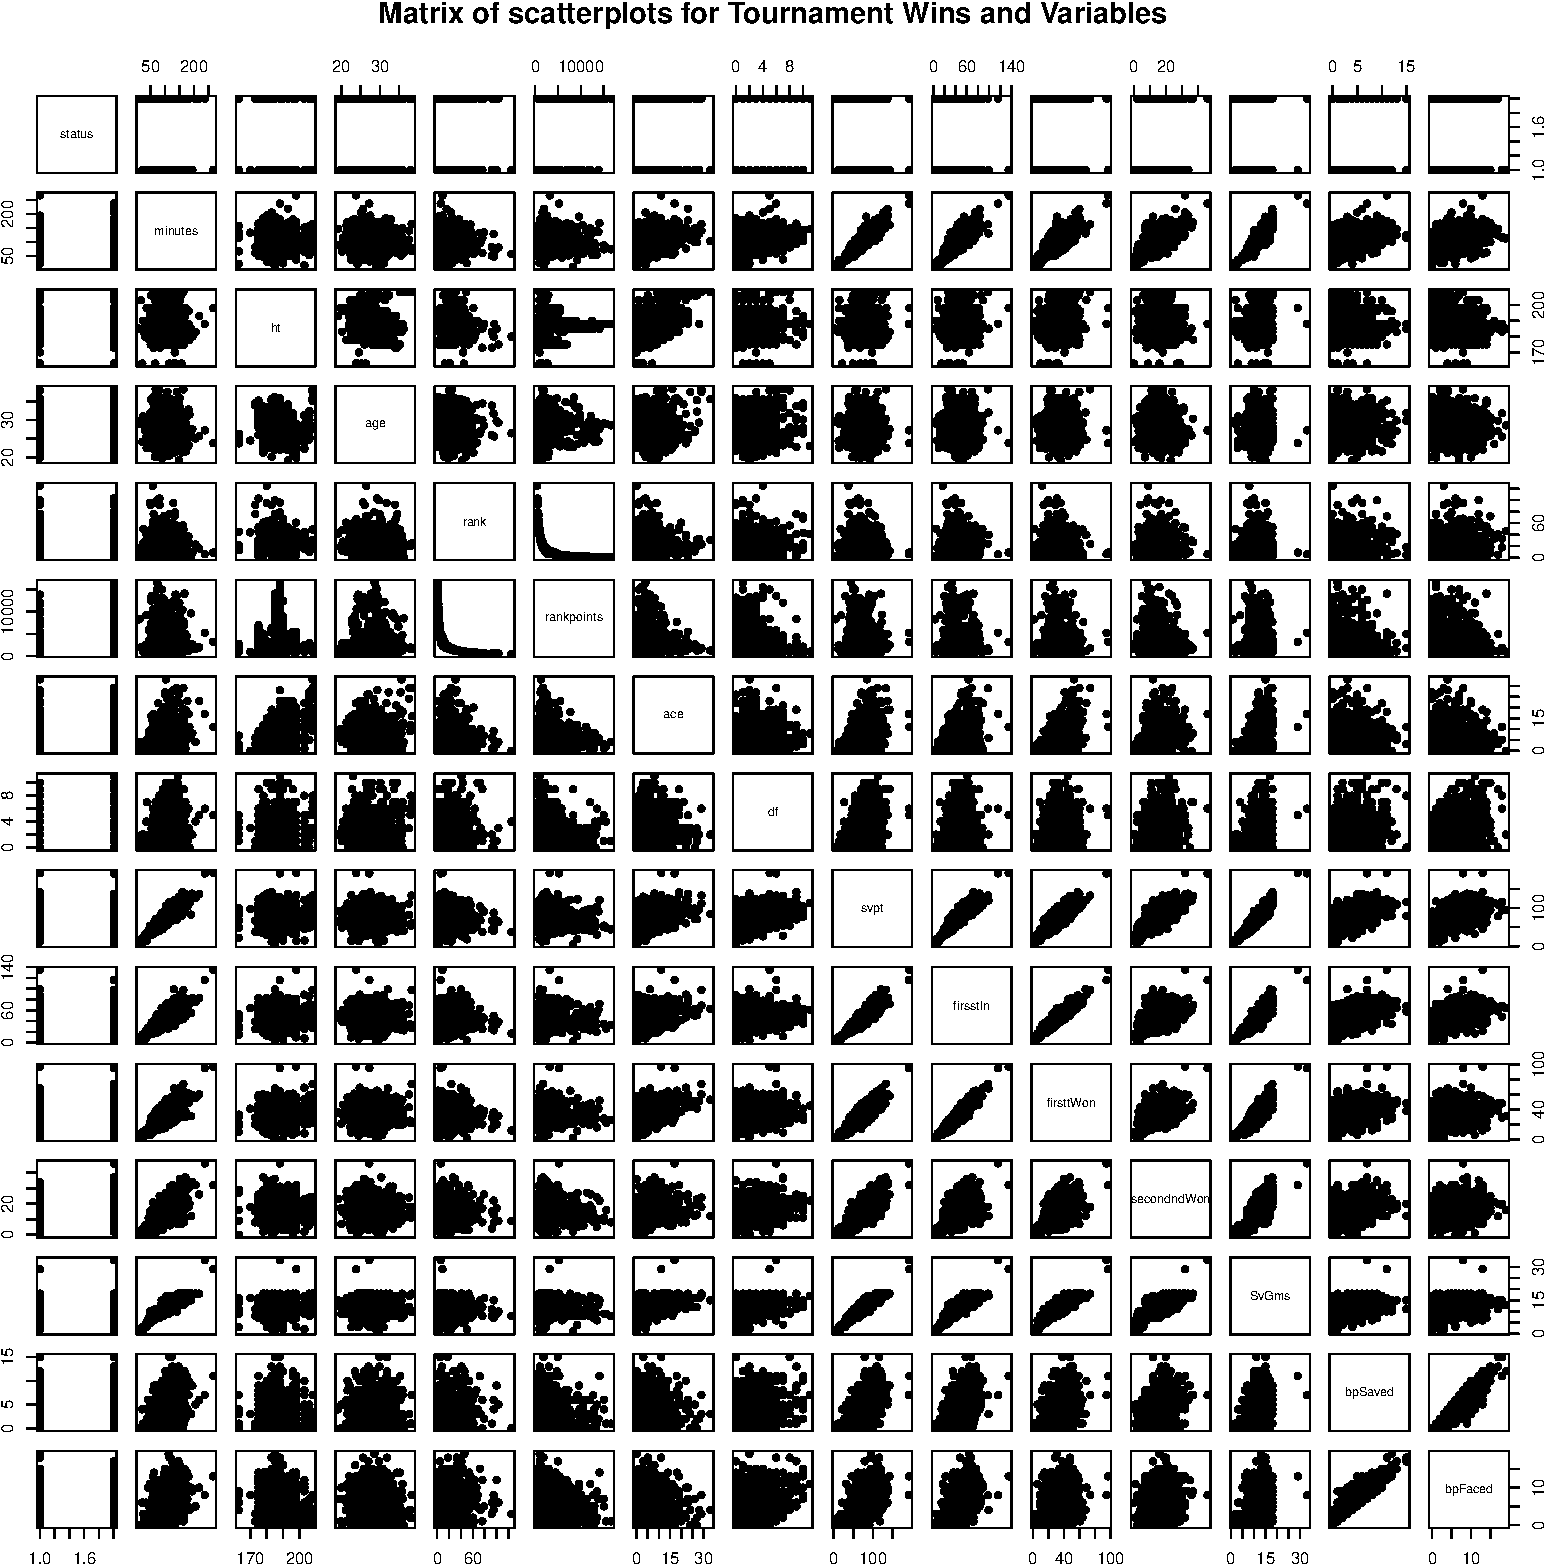
\includegraphics{Project_files/figure-latex/unnamed-chunk-5-1.pdf}

Looking at the matrix plot, we will already consider removing the
following favirables because of multicollinearity: \texttt{svpt},
\texttt{firsstIn}, \texttt{firsttWon}, \texttt{secondndWon},
\texttt{SvGms}, and \texttt{bpFaced}.

We will now look at box plots of the numeric variables we will include
in our full model:

\begin{Shaded}
\begin{Highlighting}[]
\NormalTok{p1 <-}\StringTok{ }\KeywordTok{ggplot}\NormalTok{(}\DataTypeTok{data=}\NormalTok{ten,}\KeywordTok{aes}\NormalTok{(}\DataTypeTok{x=}\NormalTok{status,}\DataTypeTok{y=}\NormalTok{minutes, }\DataTypeTok{group=}\NormalTok{status)) }\OperatorTok{+}
\StringTok{  }\KeywordTok{geom_boxplot}\NormalTok{() }\OperatorTok{+}\StringTok{ }
\StringTok{  }\KeywordTok{labs}\NormalTok{(}\DataTypeTok{title=}\StringTok{"Minutes by Status"}\NormalTok{,}
       \DataTypeTok{x =} \StringTok{"0 if Lost, 1 if Won"}\NormalTok{,}
       \DataTypeTok{y =} \StringTok{"Minutes"}\NormalTok{)}
\NormalTok{p2 <-}\StringTok{ }\KeywordTok{ggplot}\NormalTok{(}\DataTypeTok{data=}\NormalTok{ten,}\KeywordTok{aes}\NormalTok{(}\DataTypeTok{x=}\NormalTok{status,}\DataTypeTok{y=}\NormalTok{ht, }\DataTypeTok{group=}\NormalTok{status)) }\OperatorTok{+}
\StringTok{  }\KeywordTok{geom_boxplot}\NormalTok{() }\OperatorTok{+}\StringTok{ }
\StringTok{  }\KeywordTok{labs}\NormalTok{(}\DataTypeTok{title=}\StringTok{"Height by Status"}\NormalTok{,}
       \DataTypeTok{x =} \StringTok{"0 if Lost, 1 if Won"}\NormalTok{,}
       \DataTypeTok{y =} \StringTok{"Height"}\NormalTok{)}
\NormalTok{p3 <-}\StringTok{ }\KeywordTok{ggplot}\NormalTok{(}\DataTypeTok{data=}\NormalTok{ten,}\KeywordTok{aes}\NormalTok{(}\DataTypeTok{x=}\NormalTok{status,}\DataTypeTok{y=}\NormalTok{age, }\DataTypeTok{group=}\NormalTok{status)) }\OperatorTok{+}
\StringTok{  }\KeywordTok{geom_boxplot}\NormalTok{() }\OperatorTok{+}\StringTok{ }
\StringTok{  }\KeywordTok{labs}\NormalTok{(}\DataTypeTok{title=}\StringTok{"Age by Status"}\NormalTok{,}
       \DataTypeTok{x =} \StringTok{"0 if Lost, 1 if Won"}\NormalTok{,}
       \DataTypeTok{y =} \StringTok{"Age (years)"}\NormalTok{)}
\NormalTok{p4 <-}\StringTok{ }\KeywordTok{ggplot}\NormalTok{(}\DataTypeTok{data=}\NormalTok{ten,}\KeywordTok{aes}\NormalTok{(}\DataTypeTok{x=}\NormalTok{status,}\DataTypeTok{y=}\NormalTok{rank, }\DataTypeTok{group=}\NormalTok{status)) }\OperatorTok{+}
\StringTok{  }\KeywordTok{geom_boxplot}\NormalTok{() }\OperatorTok{+}\StringTok{ }
\StringTok{  }\KeywordTok{labs}\NormalTok{(}\DataTypeTok{title=}\StringTok{"Ranking by Status"}\NormalTok{,}
       \DataTypeTok{x =} \StringTok{"0 if Lost, 1 if Won"}\NormalTok{,}
       \DataTypeTok{y =} \StringTok{"Rank"}\NormalTok{)}
\NormalTok{p5 <-}\StringTok{ }\KeywordTok{ggplot}\NormalTok{(}\DataTypeTok{data=}\NormalTok{ten,}\KeywordTok{aes}\NormalTok{(}\DataTypeTok{x=}\NormalTok{status,}\DataTypeTok{y=}\NormalTok{rankpoints, }\DataTypeTok{group=}\NormalTok{status)) }\OperatorTok{+}
\StringTok{  }\KeywordTok{geom_boxplot}\NormalTok{() }\OperatorTok{+}\StringTok{ }
\StringTok{  }\KeywordTok{labs}\NormalTok{(}\DataTypeTok{title=}\StringTok{"Rankpoints by Status"}\NormalTok{,}
       \DataTypeTok{x =} \StringTok{"0 if Lost, 1 if Won"}\NormalTok{,}
       \DataTypeTok{y =} \StringTok{"Rankpoints"}\NormalTok{)}
\NormalTok{p6 <-}\StringTok{ }\KeywordTok{ggplot}\NormalTok{(}\DataTypeTok{data=}\NormalTok{ten,}\KeywordTok{aes}\NormalTok{(}\DataTypeTok{x=}\NormalTok{status,}\DataTypeTok{y=}\NormalTok{ace, }\DataTypeTok{group=}\NormalTok{status)) }\OperatorTok{+}
\StringTok{  }\KeywordTok{geom_boxplot}\NormalTok{() }\OperatorTok{+}\StringTok{ }
\StringTok{  }\KeywordTok{labs}\NormalTok{(}\DataTypeTok{title=}\StringTok{"Aces by Status"}\NormalTok{,}
       \DataTypeTok{x =} \StringTok{"0 if Lost, 1 if Won"}\NormalTok{,}
       \DataTypeTok{y =} \StringTok{"Aces"}\NormalTok{)}
\NormalTok{p7 <-}\StringTok{ }\KeywordTok{ggplot}\NormalTok{(}\DataTypeTok{data=}\NormalTok{ten,}\KeywordTok{aes}\NormalTok{(}\DataTypeTok{x=}\NormalTok{status,}\DataTypeTok{y=}\NormalTok{df, }\DataTypeTok{group=}\NormalTok{status)) }\OperatorTok{+}
\StringTok{  }\KeywordTok{geom_boxplot}\NormalTok{() }\OperatorTok{+}\StringTok{ }
\StringTok{  }\KeywordTok{labs}\NormalTok{(}\DataTypeTok{title=}\StringTok{"Double Faults by Status"}\NormalTok{,}
       \DataTypeTok{x =} \StringTok{"0 if Lost, 1 if Won"}\NormalTok{,}
       \DataTypeTok{y =} \StringTok{"Double Faults"}\NormalTok{)}
\NormalTok{p8 <-}\StringTok{ }\KeywordTok{ggplot}\NormalTok{(}\DataTypeTok{data=}\NormalTok{ten,}\KeywordTok{aes}\NormalTok{(}\DataTypeTok{x=}\NormalTok{status,}\DataTypeTok{y=}\NormalTok{bpSaved, }\DataTypeTok{group=}\NormalTok{status)) }\OperatorTok{+}
\StringTok{  }\KeywordTok{geom_boxplot}\NormalTok{() }\OperatorTok{+}\StringTok{ }
\StringTok{  }\KeywordTok{labs}\NormalTok{(}\DataTypeTok{title=}\StringTok{"Saved Breakpoints by Status"}\NormalTok{,}
       \DataTypeTok{x =} \StringTok{"0 if Lost, 1 if Won"}\NormalTok{,}
       \DataTypeTok{y =} \StringTok{"Saved Breakpoints"}\NormalTok{)}

\KeywordTok{plot_grid}\NormalTok{(p1,p2,p3,p4,p5,}
\NormalTok{          p6,p7,p8,}\DataTypeTok{ncol=}\DecValTok{2}\NormalTok{)}
\end{Highlighting}
\end{Shaded}

\includegraphics{Project_files/figure-latex/unnamed-chunk-6-1.pdf}

And we will include a stacked bar graph for the variable
\texttt{surface}.

\begin{Shaded}
\begin{Highlighting}[]
\KeywordTok{ggplot}\NormalTok{(}\DataTypeTok{data=}\NormalTok{ten,}\KeywordTok{aes}\NormalTok{(}\DataTypeTok{x=}\NormalTok{surface, }\DataTypeTok{fill =}\NormalTok{ status)) }\OperatorTok{+}\StringTok{ }\KeywordTok{geom_bar}\NormalTok{(}\DataTypeTok{position =} \StringTok{"fill"}\NormalTok{) }\OperatorTok{+}\StringTok{ }
\StringTok{  }\KeywordTok{labs}\NormalTok{(}\DataTypeTok{title=}\StringTok{"Status vs. Surface"}\NormalTok{)}
\end{Highlighting}
\end{Shaded}

\includegraphics{Project_files/figure-latex/unnamed-chunk-7-1.pdf}

In looking at all of these observations, it seems like the medians of
the numeric distributions do not seem to differ that much by status of
winning or losing. The same can be said about the proportions of winning
and losing matches against all three surfaces. In creating our model, it
could be difficult to see which variables could be helpful in
differentiating between whether a player will win a match or not. But,
we hope to see that a combination of these variables will be helpful in
determining a model that best predicts the percentage of winning a
match.

\hypertarget{logistic-regression-model}{%
\section{Logistic Regression Model}\label{logistic-regression-model}}

To begin our regression models, we will use all of the variables we
deemed important from our exploratory data analysis.

\begin{Shaded}
\begin{Highlighting}[]
\NormalTok{full_model <-}\StringTok{ }\KeywordTok{glm}\NormalTok{(status }\OperatorTok{~}\StringTok{ }\NormalTok{minutes }\OperatorTok{+}\StringTok{ }\NormalTok{ht }\OperatorTok{+}\StringTok{ }\NormalTok{age }\OperatorTok{+}\StringTok{ }\NormalTok{rank }\OperatorTok{+}\StringTok{ }
\StringTok{                }\NormalTok{rankpoints }\OperatorTok{+}\StringTok{ }\NormalTok{ace }\OperatorTok{+}\StringTok{ }\NormalTok{df }\OperatorTok{+}\StringTok{ }\NormalTok{bpSaved }\OperatorTok{+}\StringTok{ }\NormalTok{surface, }
                \DataTypeTok{family=}\NormalTok{binomial,}\DataTypeTok{data=}\NormalTok{ten)}
\KeywordTok{kable}\NormalTok{(}\KeywordTok{tidy}\NormalTok{(full_model), }\DataTypeTok{format=}\StringTok{"markdown"}\NormalTok{, }\DataTypeTok{digits =} \DecValTok{3}\NormalTok{)}
\end{Highlighting}
\end{Shaded}

\begin{longtable}[]{@{}lrrrr@{}}
\toprule
term & estimate & std.error & statistic & p.value\tabularnewline
\midrule
\endhead
(Intercept) & 5.060 & 2.219 & 2.280 & 0.023\tabularnewline
minutes & -0.007 & 0.003 & -2.607 & 0.009\tabularnewline
ht & -0.024 & 0.011 & -2.278 & 0.023\tabularnewline
age & 0.024 & 0.022 & 1.085 & 0.278\tabularnewline
rank & -0.002 & 0.006 & -0.279 & 0.780\tabularnewline
rankpoints & 0.000 & 0.000 & 3.963 & 0.000\tabularnewline
ace & 0.108 & 0.019 & 5.674 & 0.000\tabularnewline
df & -0.140 & 0.037 & -3.830 & 0.000\tabularnewline
bpSaved & -0.077 & 0.029 & -2.650 & 0.008\tabularnewline
surfaceGrass & -0.580 & 0.280 & -2.076 & 0.038\tabularnewline
surfaceHard & -0.494 & 0.165 & -3.000 & 0.003\tabularnewline
\bottomrule
\end{longtable}

\begin{Shaded}
\begin{Highlighting}[]
\NormalTok{full_w_interactions <-}\StringTok{ }\KeywordTok{glm}\NormalTok{(status }\OperatorTok{~}\StringTok{ }\NormalTok{minutes }\OperatorTok{+}\StringTok{ }\NormalTok{ht }\OperatorTok{+}\StringTok{ }\NormalTok{age }\OperatorTok{+}\StringTok{ }\NormalTok{rank }\OperatorTok{+}\StringTok{ }
\StringTok{                }\NormalTok{rankpoints }\OperatorTok{+}\StringTok{ }\NormalTok{ace }\OperatorTok{+}\StringTok{ }\NormalTok{df }\OperatorTok{+}\StringTok{ }\NormalTok{bpSaved }\OperatorTok{+}\StringTok{ }\NormalTok{surface }\OperatorTok{+}\StringTok{ }\NormalTok{surface }\OperatorTok{*}\StringTok{ }\NormalTok{minutes }\OperatorTok{+}
\StringTok{                }\NormalTok{surface }\OperatorTok{*}\StringTok{ }\NormalTok{ht }\OperatorTok{+}\StringTok{ }\NormalTok{surface }\OperatorTok{*}\StringTok{ }\NormalTok{age }\OperatorTok{+}\StringTok{ }\NormalTok{surface }\OperatorTok{*}\StringTok{ }\NormalTok{rank }\OperatorTok{+}\StringTok{ }\NormalTok{surface }\OperatorTok{*}\StringTok{ }\NormalTok{rankpoints }\OperatorTok{+}\StringTok{ }
\StringTok{                }\NormalTok{surface }\OperatorTok{*}\StringTok{ }\NormalTok{ace }\OperatorTok{+}\StringTok{ }\NormalTok{surface }\OperatorTok{*}\StringTok{ }\NormalTok{df }\OperatorTok{+}\StringTok{ }\NormalTok{surface }\OperatorTok{*}\StringTok{ }\NormalTok{bpSaved,}
                \DataTypeTok{family=}\NormalTok{binomial,}\DataTypeTok{data=}\NormalTok{ten)}
\end{Highlighting}
\end{Shaded}

\begin{Shaded}
\begin{Highlighting}[]
\KeywordTok{tidy}\NormalTok{(}\KeywordTok{anova}\NormalTok{(full_model, full_w_interactions, }\DataTypeTok{test =} \StringTok{"Chisq"}\NormalTok{))}
\end{Highlighting}
\end{Shaded}

\begin{verbatim}
## Warning in tidy.anova(anova(full_model, full_w_interactions, test =
## "Chisq")): The following column names in ANOVA output were not recognized
## or transformed: Resid..Df, Resid..Dev, Deviance
\end{verbatim}

\begin{verbatim}
## Warning: Unknown or uninitialised column: 'term'.
\end{verbatim}

\begin{verbatim}
## # A tibble: 2 x 5
##   Resid..Df Resid..Dev    df Deviance p.value
## *     <dbl>      <dbl> <dbl>    <dbl>   <dbl>
## 1       989      1176.    NA     NA   NA     
## 2       973      1149.    16     26.6  0.0457
\end{verbatim}

\begin{Shaded}
\begin{Highlighting}[]
\NormalTok{model.selected.interactions <-}\StringTok{ }\KeywordTok{step}\NormalTok{(full_w_interactions,}\DataTypeTok{direction=}\StringTok{"backward"}\NormalTok{)}
\end{Highlighting}
\end{Shaded}

\begin{verbatim}
## Start:  AIC=1202.97
## status ~ minutes + ht + age + rank + rankpoints + ace + df + 
##     bpSaved + surface + surface * minutes + surface * ht + surface * 
##     age + surface * rank + surface * rankpoints + surface * ace + 
##     surface * df + surface * bpSaved
## 
##                      Df Deviance    AIC
## - rank:surface        2   1149.4 1199.4
## - age:surface         2   1150.3 1200.3
## - bpSaved:surface     2   1150.5 1200.5
## - rankpoints:surface  2   1150.5 1200.5
## - minutes:surface     2   1150.6 1200.6
## <none>                    1149.0 1203.0
## - df:surface          2   1154.7 1204.7
## - ht:surface          2   1154.7 1204.7
## - ace:surface         2   1156.9 1206.9
## 
## Step:  AIC=1199.39
## status ~ minutes + ht + age + rank + rankpoints + ace + df + 
##     bpSaved + surface + minutes:surface + ht:surface + age:surface + 
##     rankpoints:surface + ace:surface + df:surface + bpSaved:surface
## 
##                      Df Deviance    AIC
## - bpSaved:surface     2   1150.7 1196.7
## - age:surface         2   1150.8 1196.8
## - minutes:surface     2   1150.9 1196.9
## - rankpoints:surface  2   1151.1 1197.1
## - rank                1   1149.6 1197.6
## <none>                    1149.4 1199.4
## - ht:surface          2   1154.8 1200.8
## - df:surface          2   1154.8 1200.8
## - ace:surface         2   1157.6 1203.6
## 
## Step:  AIC=1196.71
## status ~ minutes + ht + age + rank + rankpoints + ace + df + 
##     bpSaved + surface + minutes:surface + ht:surface + age:surface + 
##     rankpoints:surface + ace:surface + df:surface
## 
##                      Df Deviance    AIC
## - minutes:surface     2   1151.6 1193.6
## - age:surface         2   1151.9 1193.9
## - rankpoints:surface  2   1152.4 1194.4
## - rank                1   1150.9 1194.9
## <none>                    1150.7 1196.7
## - ht:surface          2   1156.4 1198.4
## - ace:surface         2   1158.1 1200.1
## - bpSaved             1   1156.8 1200.8
## - df:surface          2   1159.6 1201.6
## 
## Step:  AIC=1193.59
## status ~ minutes + ht + age + rank + rankpoints + ace + df + 
##     bpSaved + surface + ht:surface + age:surface + rankpoints:surface + 
##     ace:surface + df:surface
## 
##                      Df Deviance    AIC
## - age:surface         2   1153.0 1191.0
## - rankpoints:surface  2   1153.7 1191.7
## - rank                1   1151.8 1191.8
## <none>                    1151.6 1193.6
## - ht:surface          2   1156.8 1194.8
## - ace:surface         2   1158.4 1196.4
## - bpSaved             1   1157.6 1197.6
## - df:surface          2   1160.4 1198.4
## - minutes             1   1159.3 1199.3
## 
## Step:  AIC=1190.98
## status ~ minutes + ht + age + rank + rankpoints + ace + df + 
##     bpSaved + surface + ht:surface + rankpoints:surface + ace:surface + 
##     df:surface
## 
##                      Df Deviance    AIC
## - rankpoints:surface  2   1154.9 1188.9
## - rank                1   1153.2 1189.2
## - age                 1   1153.5 1189.5
## <none>                    1153.0 1191.0
## - ht:surface          2   1158.7 1192.7
## - ace:surface         2   1160.6 1194.6
## - bpSaved             1   1159.2 1195.2
## - df:surface          2   1162.2 1196.2
## - minutes             1   1160.8 1196.8
## 
## Step:  AIC=1188.92
## status ~ minutes + ht + age + rank + rankpoints + ace + df + 
##     bpSaved + surface + ht:surface + ace:surface + df:surface
## 
##               Df Deviance    AIC
## - rank         1   1155.1 1187.1
## - age          1   1155.5 1187.5
## <none>             1154.9 1188.9
## - ht:surface   2   1160.6 1190.6
## - ace:surface  2   1162.5 1192.5
## - bpSaved      1   1161.3 1193.3
## - minutes      1   1162.9 1194.9
## - df:surface   2   1164.9 1194.9
## - rankpoints   1   1173.8 1205.8
## 
## Step:  AIC=1187.07
## status ~ minutes + ht + age + rankpoints + ace + df + bpSaved + 
##     surface + ht:surface + ace:surface + df:surface
## 
##               Df Deviance    AIC
## - age          1   1155.6 1185.6
## <none>             1155.1 1187.1
## - ht:surface   2   1160.7 1188.7
## - ace:surface  2   1162.7 1190.7
## - bpSaved      1   1161.7 1191.7
## - minutes      1   1162.9 1192.9
## - df:surface   2   1165.1 1193.1
## - rankpoints   1   1193.0 1223.0
## 
## Step:  AIC=1185.62
## status ~ minutes + ht + rankpoints + ace + df + bpSaved + surface + 
##     ht:surface + ace:surface + df:surface
## 
##               Df Deviance    AIC
## <none>             1155.6 1185.6
## - ht:surface   2   1161.4 1187.4
## - ace:surface  2   1163.5 1189.5
## - bpSaved      1   1162.1 1190.1
## - minutes      1   1163.8 1191.8
## - df:surface   2   1165.8 1191.8
## - rankpoints   1   1193.6 1221.6
\end{verbatim}

\hypertarget{model}{%
\section{Model}\label{model}}

\begin{Shaded}
\begin{Highlighting}[]
\NormalTok{final.base.model <-}\StringTok{ }\NormalTok{model.selected.interactions}
\KeywordTok{kable}\NormalTok{(}\KeywordTok{tidy}\NormalTok{(final.base.model), }\DataTypeTok{format =} \StringTok{"markdown"}\NormalTok{, }\DataTypeTok{digits =} \DecValTok{3}\NormalTok{)}
\end{Highlighting}
\end{Shaded}

\begin{longtable}[]{@{}lrrrr@{}}
\toprule
term & estimate & std.error & statistic & p.value\tabularnewline
\midrule
\endhead
(Intercept) & 10.392 & 3.518 & 2.954 & 0.003\tabularnewline
minutes & -0.008 & 0.003 & -2.844 & 0.004\tabularnewline
ht & -0.048 & 0.019 & -2.547 & 0.011\tabularnewline
rankpoints & 0.000 & 0.000 & 5.441 & 0.000\tabularnewline
ace & 0.110 & 0.040 & 2.764 & 0.006\tabularnewline
df & -0.243 & 0.070 & -3.474 & 0.001\tabularnewline
bpSaved & -0.075 & 0.029 & -2.548 & 0.011\tabularnewline
surfaceGrass & 5.285 & 8.299 & 0.637 & 0.524\tabularnewline
surfaceHard & -8.048 & 4.294 & -1.874 & 0.061\tabularnewline
ht:surfaceGrass & -0.043 & 0.045 & -0.940 & 0.347\tabularnewline
ht:surfaceHard & 0.040 & 0.023 & 1.710 & 0.087\tabularnewline
ace:surfaceGrass & 0.164 & 0.080 & 2.048 & 0.041\tabularnewline
ace:surfaceHard & -0.021 & 0.045 & -0.469 & 0.639\tabularnewline
df:surfaceGrass & 0.425 & 0.132 & 3.205 & 0.001\tabularnewline
df:surfaceHard & 0.107 & 0.082 & 1.297 & 0.195\tabularnewline
\bottomrule
\end{longtable}

\hypertarget{model-assessment}{%
\section{Model Assessment}\label{model-assessment}}

\hypertarget{binned-plots-with-residuals-vs-predicted}{%
\subsection{Binned Plots with Residuals vs
Predicted}\label{binned-plots-with-residuals-vs-predicted}}

\begin{Shaded}
\begin{Highlighting}[]
\NormalTok{ten <-}\StringTok{ }\NormalTok{ten }\OperatorTok\StringTok{ }\KeywordTok{mutate}\NormalTok{(}\DataTypeTok{Residuals =} \KeywordTok{residuals.glm}\NormalTok{(final.base.model,}\DataTypeTok{type=}\StringTok{"response"}\NormalTok{),}
                          \DataTypeTok{Predicted =} \KeywordTok{predict.glm}\NormalTok{(final.base.model,}\DataTypeTok{type=}\StringTok{"response"}\NormalTok{))}

\KeywordTok{binnedplot}\NormalTok{(ten}\OperatorTok{$}\NormalTok{Predicted, ten}\OperatorTok{$}\NormalTok{Residuals,}\DataTypeTok{xlab=}\StringTok{"Predicted Probabilities"}\NormalTok{,}
           \DataTypeTok{ylab=}\StringTok{"Residuals"}\NormalTok{,}\DataTypeTok{main=}\StringTok{"Binned Residuals vs. Predicted Probabilities"}\NormalTok{)}
\end{Highlighting}
\end{Shaded}

\includegraphics{Project_files/figure-latex/unnamed-chunk-13-1.pdf}

\includegraphics{Project_files/figure-latex/unnamed-chunk-14-1.pdf}
\includegraphics{Project_files/figure-latex/unnamed-chunk-14-2.pdf}
\includegraphics{Project_files/figure-latex/unnamed-chunk-14-3.pdf}
\includegraphics{Project_files/figure-latex/unnamed-chunk-14-4.pdf}
\includegraphics{Project_files/figure-latex/unnamed-chunk-14-5.pdf}
\includegraphics{Project_files/figure-latex/unnamed-chunk-14-6.pdf}

\begin{Shaded}
\begin{Highlighting}[]
\NormalTok{ROC.ten <-}\StringTok{ }\KeywordTok{roc}\NormalTok{(ten}\OperatorTok{$}\NormalTok{status,ten}\OperatorTok{$}\NormalTok{Predicted,}\DataTypeTok{plot=}\NormalTok{T)}
\end{Highlighting}
\end{Shaded}

\includegraphics{Project_files/figure-latex/unnamed-chunk-15-1.pdf}

\begin{Shaded}
\begin{Highlighting}[]
\NormalTok{ROC.ten}\OperatorTok{$}\NormalTok{auc}
\end{Highlighting}
\end{Shaded}

\begin{verbatim}
## Area under the curve: 0.7268
\end{verbatim}

\begin{Shaded}
\begin{Highlighting}[]
\NormalTok{threshold =}\StringTok{ }\FloatTok{0.30}
\KeywordTok{table}\NormalTok{(ten}\OperatorTok{$}\NormalTok{status, ten}\OperatorTok{$}\NormalTok{Predicted }\OperatorTok{>}\StringTok{ }\NormalTok{threshold)}
\end{Highlighting}
\end{Shaded}

\begin{verbatim}
##    
##     FALSE TRUE
##   0    26  326
##   1    13  635
\end{verbatim}

\begin{Shaded}
\begin{Highlighting}[]
\NormalTok{(}\DecValTok{326} \OperatorTok{+}\StringTok{ }\DecValTok{13}\NormalTok{)}\OperatorTok{/}\NormalTok{(}\DecValTok{26}\OperatorTok{+}\DecValTok{13}\OperatorTok{+}\DecValTok{326}\OperatorTok{+}\DecValTok{635}\NormalTok{)}
\end{Highlighting}
\end{Shaded}

\begin{verbatim}
## [1] 0.339
\end{verbatim}

\hypertarget{influential-points}{%
\section{Influential Points}\label{influential-points}}

\hypertarget{vif}{%
\subsection{VIF}\label{vif}}

\begin{Shaded}
\begin{Highlighting}[]
\KeywordTok{tidy}\NormalTok{(}\KeywordTok{vif}\NormalTok{(final.base.model))}
\end{Highlighting}
\end{Shaded}

\begin{verbatim}
## Warning: 'tidy.matrix' is deprecated.
## See help("Deprecated")
\end{verbatim}

\begin{verbatim}
## # A tibble: 10 x 4
##    .rownames        GVIF    Df GVIF..1..2.Df..
##    <chr>           <dbl> <dbl>           <dbl>
##  1 minutes          1.45     1            1.21
##  2 ht               3.99     1            2.00
##  3 rankpoints       1.04     1            1.02
##  4 ace              6.82     1            2.61
##  5 df               4.02     1            2.00
##  6 bpSaved          1.32     1            1.15
##  7 surface     650920.       2           28.4 
##  8 ht:surface  721588.       2           29.1 
##  9 ace:surface     43.8      2            2.57
## 10 df:surface      14.7      2            1.96
\end{verbatim}

After looking at the VIF values, we see that the VIF for
\texttt{surface} is greater than 10, so we will also remove it from the
model. This means we will also have to remove the interaction variables
as well.

\hypertarget{linear-regression-assumptions-revised}{%
\section{Linear Regression Assumptions:
Revised}\label{linear-regression-assumptions-revised}}

Because one of our residuals plots has a non-linear relationship, we
will remove \texttt{bpSaved} from the model and redo the assumptions. We
will also remove \texttt{surface} and its corresponding interactions
effects.

\begin{Shaded}
\begin{Highlighting}[]
\NormalTok{newten <-}\StringTok{ }\NormalTok{ten}
\NormalTok{final <-}\StringTok{ }\KeywordTok{glm}\NormalTok{(status }\OperatorTok{~}\StringTok{ }\NormalTok{minutes }\OperatorTok{+}\StringTok{ }\NormalTok{ht }\OperatorTok{+}\StringTok{ }\NormalTok{rankpoints }\OperatorTok{+}\StringTok{ }\NormalTok{ace }\OperatorTok{+}\StringTok{ }\NormalTok{df, }\DataTypeTok{family =}\NormalTok{ binomial, }\DataTypeTok{data =}\NormalTok{ newten)}
\KeywordTok{kable}\NormalTok{(}\KeywordTok{tidy}\NormalTok{(final), }\DataTypeTok{format =} \StringTok{"markdown"}\NormalTok{, }\DataTypeTok{digits =} \DecValTok{3}\NormalTok{)}
\end{Highlighting}
\end{Shaded}

\begin{longtable}[]{@{}lrrrr@{}}
\toprule
term & estimate & std.error & statistic & p.value\tabularnewline
\midrule
\endhead
(Intercept) & 5.197 & 1.951 & 2.664 & 0.008\tabularnewline
minutes & -0.009 & 0.002 & -3.715 & 0.000\tabularnewline
ht & -0.023 & 0.010 & -2.221 & 0.026\tabularnewline
rankpoints & 0.000 & 0.000 & 5.238 & 0.000\tabularnewline
ace & 0.094 & 0.018 & 5.371 & 0.000\tabularnewline
df & -0.169 & 0.036 & -4.770 & 0.000\tabularnewline
\bottomrule
\end{longtable}

\begin{Shaded}
\begin{Highlighting}[]
\KeywordTok{pairs}\NormalTok{(status }\OperatorTok{~}\StringTok{ }\NormalTok{minutes }\OperatorTok{+}\StringTok{ }\NormalTok{ht }\OperatorTok{+}\StringTok{ }\NormalTok{rankpoints }\OperatorTok{+}\StringTok{ }\NormalTok{ace }\OperatorTok{+}\StringTok{ }\NormalTok{df, }\DataTypeTok{data =}\NormalTok{ newten)}
\end{Highlighting}
\end{Shaded}

\includegraphics{Project_files/figure-latex/unnamed-chunk-21-1.pdf}

The scatterplot matrix does not show obvious signs of multicollinearity.

\hypertarget{model-assessment-1}{%
\section{Model Assessment}\label{model-assessment-1}}

\hypertarget{binned-plots-with-residuals-vs-predicted-1}{%
\subsection{Binned Plots with Residuals vs
Predicted}\label{binned-plots-with-residuals-vs-predicted-1}}

\begin{Shaded}
\begin{Highlighting}[]
\NormalTok{newten <-}\StringTok{ }\NormalTok{newten }\OperatorTok\StringTok{ }\KeywordTok{mutate}\NormalTok{(}\DataTypeTok{Residuals =} \KeywordTok{residuals.glm}\NormalTok{(final,}\DataTypeTok{type=}\StringTok{"response"}\NormalTok{),}
                          \DataTypeTok{Predicted =} \KeywordTok{predict.glm}\NormalTok{(final,}\DataTypeTok{type=}\StringTok{"response"}\NormalTok{))}

\KeywordTok{binnedplot}\NormalTok{(newten}\OperatorTok{$}\NormalTok{Predicted, newten}\OperatorTok{$}\NormalTok{Residuals,}\DataTypeTok{xlab=}\StringTok{"Predicted Probabilities"}\NormalTok{,}
           \DataTypeTok{ylab=}\StringTok{"Residuals"}\NormalTok{,}\DataTypeTok{main=}\StringTok{"Binned Residuals vs. Predicted Probabilities"}\NormalTok{)}
\end{Highlighting}
\end{Shaded}

\includegraphics{Project_files/figure-latex/unnamed-chunk-22-1.pdf}

\includegraphics{Project_files/figure-latex/unnamed-chunk-23-1.pdf}
\includegraphics{Project_files/figure-latex/unnamed-chunk-23-2.pdf}
\includegraphics{Project_files/figure-latex/unnamed-chunk-23-3.pdf}
\includegraphics{Project_files/figure-latex/unnamed-chunk-23-4.pdf}
\includegraphics{Project_files/figure-latex/unnamed-chunk-23-5.pdf}

\begin{Shaded}
\begin{Highlighting}[]
\NormalTok{ROC.newten <-}\StringTok{ }\KeywordTok{roc}\NormalTok{(newten}\OperatorTok{$}\NormalTok{status,newten}\OperatorTok{$}\NormalTok{Predicted,}\DataTypeTok{plot=}\NormalTok{T)}
\end{Highlighting}
\end{Shaded}

\includegraphics{Project_files/figure-latex/unnamed-chunk-24-1.pdf}

\begin{Shaded}
\begin{Highlighting}[]
\NormalTok{ROC.newten}\OperatorTok{$}\NormalTok{auc}
\end{Highlighting}
\end{Shaded}

\begin{verbatim}
## Area under the curve: 0.6996
\end{verbatim}

\begin{Shaded}
\begin{Highlighting}[]
\NormalTok{threshold =}\StringTok{ }\FloatTok{0.30}
\KeywordTok{table}\NormalTok{(newten}\OperatorTok{$}\NormalTok{status, newten}\OperatorTok{$}\NormalTok{Predicted }\OperatorTok{>}\StringTok{ }\NormalTok{threshold)}
\end{Highlighting}
\end{Shaded}

\begin{verbatim}
##    
##     FALSE TRUE
##   0    10  342
##   1    10  638
\end{verbatim}

\begin{Shaded}
\begin{Highlighting}[]
\NormalTok{(}\DecValTok{342} \OperatorTok{+}\StringTok{ }\DecValTok{10}\NormalTok{)}\OperatorTok{/}\NormalTok{(}\DecValTok{342} \OperatorTok{+}\StringTok{ }\DecValTok{10} \OperatorTok{+}\StringTok{ }\DecValTok{10} \OperatorTok{+}\StringTok{ }\DecValTok{638}\NormalTok{)}
\end{Highlighting}
\end{Shaded}

\begin{verbatim}
## [1] 0.352
\end{verbatim}

\hypertarget{prediction}{%
\section{Prediction}\label{prediction}}

\hypertarget{test-cases}{%
\subsection{Test cases:}\label{test-cases}}

We will look at a match that was played the Monte Carlo Masters in 2014
between Roger Federer and Novak Djokovic. We want to see the probability
that a player will win the match.

\begin{Shaded}
\begin{Highlighting}[]
\NormalTok{tennis }\OperatorTok
\StringTok{  }\KeywordTok{filter}\NormalTok{(tourney_name }\OperatorTok{==}\StringTok{ "Monte Carlo Masters"}\NormalTok{,}
\NormalTok{         name }\OperatorTok{==}\StringTok{ "Roger Federer"} \OperatorTok{|}\StringTok{  }\NormalTok{name }\OperatorTok{==}\StringTok{ "Novak Djokovic"}\NormalTok{,}
\NormalTok{         tourney_id }\OperatorTok{==}\StringTok{ "2014-410"}\NormalTok{,}
\NormalTok{         loser_name }\OperatorTok{==}\StringTok{ "Novak Djokovic"}\NormalTok{)}
\end{Highlighting}
\end{Shaded}

\begin{verbatim}
## # A tibble: 2 x 66
##   tourney_id tourney_name surface draw_size tourney_level tourney_date
##   <chr>      <chr>        <chr>       <int> <chr>                <int>
## 1 2014-410   Monte Carlo~ Clay           56 M                 20140413
## 2 2014-410   Monte Carlo~ Clay           56 M                 20140413
## # ... with 60 more variables: match_num <int>, winner_id <int>,
## #   winner_seed <int>, winner_entry <chr>, winner_name <chr>,
## #   winner_hand <chr>, winner_ht <int>, winner_ioc <chr>,
## #   winner_age <dbl>, winner_rank <int>, winner_rank_points <int>,
## #   loser_id <int>, loser_seed <int>, loser_entry <chr>, loser_name <chr>,
## #   loser_hand <chr>, loser_ht <int>, loser_ioc <chr>, loser_age <dbl>,
## #   loser_rank <int>, loser_rank_points <int>, score <chr>, best_of <int>,
## #   round <chr>, minutes <int>, w_ace <int>, w_df <int>, w_svpt <int>,
## #   w_1stIn <int>, w_1stWon <int>, w_2ndWon <int>, w_SvGms <int>,
## #   w_bpSaved <int>, w_bpFaced <int>, l_ace <int>, l_df <int>,
## #   l_svpt <int>, l_1stIn <int>, l_1stWon <int>, l_2ndWon <int>,
## #   l_SvGms <int>, l_bpSaved <int>, l_bpFaced <int>, seed <int>,
## #   name <chr>, hand <chr>, ht <int>, age <dbl>, rank <int>,
## #   rankpoints <int>, ace <int>, df <int>, svpt <int>, firsstIn <int>,
## #   firsttWon <int>, secondndWon <int>, SvGms <int>, bpSaved <int>,
## #   bpFaced <int>, status <dbl>
\end{verbatim}

\begin{Shaded}
\begin{Highlighting}[]
\NormalTok{fed <-}\StringTok{ }\KeywordTok{data.frame}\NormalTok{(}\DataTypeTok{minutes =} \DecValTok{75}\NormalTok{, }\DataTypeTok{ht =} \DecValTok{185}\NormalTok{, }\DataTypeTok{rankpoints =} \DecValTok{5355}\NormalTok{ , }\DataTypeTok{ace =} \DecValTok{3}\NormalTok{ , }\DataTypeTok{df =} \DecValTok{1}\NormalTok{)}
\NormalTok{djo1 <-}\StringTok{ }\KeywordTok{data.frame}\NormalTok{(}\DataTypeTok{minutes =} \DecValTok{75}\NormalTok{, }\DataTypeTok{ht =} \DecValTok{188}\NormalTok{, }\DataTypeTok{rankpoints =} \DecValTok{11680}\NormalTok{, }\DataTypeTok{ace =} \DecValTok{2}\NormalTok{, }\DataTypeTok{df =} \DecValTok{0}\NormalTok{)}
\KeywordTok{predict}\NormalTok{(final, }\DataTypeTok{newdata=}\NormalTok{fed, }\DataTypeTok{type=}\StringTok{"response"}\NormalTok{)}
\end{Highlighting}
\end{Shaded}

\begin{verbatim}
##         1 
## 0.7937041
\end{verbatim}

\begin{Shaded}
\begin{Highlighting}[]
\KeywordTok{predict}\NormalTok{(final, }\DataTypeTok{newdata=}\NormalTok{djo1, }\DataTypeTok{type=}\StringTok{"response"}\NormalTok{)}
\end{Highlighting}
\end{Shaded}

\begin{verbatim}
##         1 
## 0.9251785
\end{verbatim}

\begin{Shaded}
\begin{Highlighting}[]
\NormalTok{predsdjo1 <-}\StringTok{ }\KeywordTok{predict}\NormalTok{(final, djo1, }\DataTypeTok{type=}\StringTok{"response"}\NormalTok{, }\DataTypeTok{se.fit=}\OtherTok{TRUE}\NormalTok{)}
\NormalTok{predsfed <-}\StringTok{ }\KeywordTok{predict}\NormalTok{(final, fed, }\DataTypeTok{type=}\StringTok{"response"}\NormalTok{, }\DataTypeTok{se.fit=}\OtherTok{TRUE}\NormalTok{)}

\NormalTok{predfdjo1 <-}\StringTok{ }\NormalTok{predsdjo1}\OperatorTok{$}\NormalTok{fit }\CommentTok{# predicted}
\NormalTok{lowerdjo1 <-}\StringTok{ }\NormalTok{predsdjo1}\OperatorTok{$}\NormalTok{fit }\OperatorTok{-}\StringTok{ }\NormalTok{(}\FloatTok{1.96}\OperatorTok{*}\NormalTok{predsdjo1}\OperatorTok{$}\NormalTok{se.fit) }\CommentTok{# lower bounds}
\NormalTok{upperdjo1 <-}\StringTok{ }\NormalTok{predsdjo1}\OperatorTok{$}\NormalTok{fit }\OperatorTok{+}\StringTok{ }\NormalTok{(}\FloatTok{1.96}\OperatorTok{*}\NormalTok{predsdjo1}\OperatorTok{$}\NormalTok{se.fit) }\CommentTok{# upper bounds}

\NormalTok{predffed <-}\StringTok{ }\NormalTok{predsfed}\OperatorTok{$}\NormalTok{fit }\CommentTok{# predicted}
\NormalTok{lowerfed <-}\StringTok{ }\NormalTok{predsfed}\OperatorTok{$}\NormalTok{fit }\OperatorTok{-}\StringTok{ }\NormalTok{(}\FloatTok{1.96}\OperatorTok{*}\NormalTok{predsfed}\OperatorTok{$}\NormalTok{se.fit) }\CommentTok{# lower bounds}
\NormalTok{upperfed <-}\StringTok{ }\NormalTok{predsfed}\OperatorTok{$}\NormalTok{fit }\OperatorTok{+}\StringTok{ }\NormalTok{(}\FloatTok{1.96}\OperatorTok{*}\NormalTok{predsfed}\OperatorTok{$}\NormalTok{se.fit) }\CommentTok{# lower bounds}

\KeywordTok{c}\NormalTok{(predfdjo1, lowerdjo1, upperdjo1)}
\end{Highlighting}
\end{Shaded}

\begin{verbatim}
##         1         1         1 
## 0.9251785 0.8782777 0.9720793
\end{verbatim}

\begin{Shaded}
\begin{Highlighting}[]
\KeywordTok{c}\NormalTok{(predffed, lowerfed, upperfed)}
\end{Highlighting}
\end{Shaded}

\begin{verbatim}
##         1         1         1 
## 0.7937041 0.7473870 0.8400212
\end{verbatim}

We see that the model predicts Roger Federer has a 79.37\% chance of
winning the match, while Novak Djokovic has a 92.52\% chance of winning
the match. This is mainly because Djokovic's rank points were almost
double that of Federer's at the time. However, Federer won the match. In
this case, we had an anomaly.

The next match we will look at was played at the China Open in 2013 and
was between Novak Djokovic and Rafael Nadal.

\begin{Shaded}
\begin{Highlighting}[]
\NormalTok{tennis }\OperatorTok
\StringTok{  }\KeywordTok{filter}\NormalTok{(name }\OperatorTok{==}\StringTok{ "Novak Djokovic"} \OperatorTok{|}\StringTok{ }\NormalTok{name }\OperatorTok{==}\StringTok{ "Rafael Nadal"}\NormalTok{,}
\NormalTok{         tourney_name }\OperatorTok{==}\StringTok{ "Beijing"}\NormalTok{,}
\NormalTok{         loser_name }\OperatorTok{==}\StringTok{ "Rafael Nadal"}\NormalTok{,}
\NormalTok{         tourney_id }\OperatorTok{==}\StringTok{ "2013-747"}\NormalTok{)}
\end{Highlighting}
\end{Shaded}

\begin{verbatim}
## # A tibble: 2 x 66
##   tourney_id tourney_name surface draw_size tourney_level tourney_date
##   <chr>      <chr>        <chr>       <int> <chr>                <int>
## 1 2013-747   Beijing      Hard           32 A                 20130930
## 2 2013-747   Beijing      Hard           32 A                 20130930
## # ... with 60 more variables: match_num <int>, winner_id <int>,
## #   winner_seed <int>, winner_entry <chr>, winner_name <chr>,
## #   winner_hand <chr>, winner_ht <int>, winner_ioc <chr>,
## #   winner_age <dbl>, winner_rank <int>, winner_rank_points <int>,
## #   loser_id <int>, loser_seed <int>, loser_entry <chr>, loser_name <chr>,
## #   loser_hand <chr>, loser_ht <int>, loser_ioc <chr>, loser_age <dbl>,
## #   loser_rank <int>, loser_rank_points <int>, score <chr>, best_of <int>,
## #   round <chr>, minutes <int>, w_ace <int>, w_df <int>, w_svpt <int>,
## #   w_1stIn <int>, w_1stWon <int>, w_2ndWon <int>, w_SvGms <int>,
## #   w_bpSaved <int>, w_bpFaced <int>, l_ace <int>, l_df <int>,
## #   l_svpt <int>, l_1stIn <int>, l_1stWon <int>, l_2ndWon <int>,
## #   l_SvGms <int>, l_bpSaved <int>, l_bpFaced <int>, seed <int>,
## #   name <chr>, hand <chr>, ht <int>, age <dbl>, rank <int>,
## #   rankpoints <int>, ace <int>, df <int>, svpt <int>, firsstIn <int>,
## #   firsttWon <int>, secondndWon <int>, SvGms <int>, bpSaved <int>,
## #   bpFaced <int>, status <dbl>
\end{verbatim}

\begin{Shaded}
\begin{Highlighting}[]
\NormalTok{djo2 <-}\StringTok{ }\KeywordTok{data.frame}\NormalTok{(}\DataTypeTok{minutes =} \DecValTok{87}\NormalTok{, }\DataTypeTok{ht =} \DecValTok{188}\NormalTok{, }\DataTypeTok{rankpoints =} \DecValTok{11120}\NormalTok{, }\DataTypeTok{ace =} \DecValTok{5}\NormalTok{, }\DataTypeTok{df =} \DecValTok{1}\NormalTok{)}
\NormalTok{nadal <-}\StringTok{ }\KeywordTok{data.frame}\NormalTok{(}\DataTypeTok{minutes =} \DecValTok{87}\NormalTok{, }\DataTypeTok{ht =} \DecValTok{185}\NormalTok{, }\DataTypeTok{rankpoints =} \DecValTok{10860}\NormalTok{, }\DataTypeTok{ace =} \DecValTok{2}\NormalTok{, }\DataTypeTok{df =} \DecValTok{2}\NormalTok{)}
\KeywordTok{predict}\NormalTok{(final, }\DataTypeTok{newdata=}\NormalTok{djo2, }\DataTypeTok{type=}\StringTok{"response"}\NormalTok{)}
\end{Highlighting}
\end{Shaded}

\begin{verbatim}
##         1 
## 0.9182071
\end{verbatim}

\begin{Shaded}
\begin{Highlighting}[]
\KeywordTok{predict}\NormalTok{(final, }\DataTypeTok{newdata=}\NormalTok{nadal, }\DataTypeTok{type=}\StringTok{"response"}\NormalTok{)}
\end{Highlighting}
\end{Shaded}

\begin{verbatim}
##         1 
## 0.8795555
\end{verbatim}

We see that the model predicts Novak Djokovic has a 91.82\% chance of
winning the match, while Rafael Nadal has a 87.96\% chance of winning
the match. Djokovic won the match.

\hypertarget{test-case-with-similar-rank-points}{%
\subsubsection{Test Case with Similar Rank
Points}\label{test-case-with-similar-rank-points}}

Now, we'll look at a match where both players had similar rank points.
The match we will look at is between Jo Wilfried Tsonga and Michael
Llodra, and was played at the Queen's Club Championships in 2011.

\begin{Shaded}
\begin{Highlighting}[]
\NormalTok{ten }\OperatorTok
\StringTok{  }\KeywordTok{filter}\NormalTok{(winner_rank_points }\OperatorTok{>}\StringTok{ }\DecValTok{1000} \OperatorTok{&}\StringTok{ }\NormalTok{winner_rank_points }\OperatorTok{<}\StringTok{ }\DecValTok{2000} \OperatorTok{&}\StringTok{ }\NormalTok{loser_rank_points }\OperatorTok{>}\StringTok{ }\DecValTok{1000} \OperatorTok{&}\StringTok{ }\NormalTok{loser_rank_points }\OperatorTok{<}\StringTok{ }\DecValTok{2000}\NormalTok{,}
\NormalTok{         tourney_id }\OperatorTok{==}\StringTok{ "2011-311"}\NormalTok{,}
\NormalTok{         tourney_name }\OperatorTok{==}\StringTok{ "Queen's Club"}\NormalTok{,}
\NormalTok{         winner_name }\OperatorTok{==}\StringTok{ "Jo Wilfried Tsonga"}
\NormalTok{         )}
\end{Highlighting}
\end{Shaded}

\begin{verbatim}
## # A tibble: 1 x 68
##   tourney_id tourney_name surface draw_size tourney_level tourney_date
##   <chr>      <chr>        <chr>       <int> <chr>                <int>
## 1 2011-311   Queen's Club Grass          56 A                 20110606
## # ... with 62 more variables: match_num <int>, winner_id <int>,
## #   winner_seed <int>, winner_entry <chr>, winner_name <chr>,
## #   winner_hand <chr>, winner_ht <int>, winner_ioc <chr>,
## #   winner_age <dbl>, winner_rank <int>, winner_rank_points <int>,
## #   loser_id <int>, loser_seed <int>, loser_entry <chr>, loser_name <chr>,
## #   loser_hand <chr>, loser_ht <int>, loser_ioc <chr>, loser_age <dbl>,
## #   loser_rank <int>, loser_rank_points <int>, score <chr>, best_of <int>,
## #   round <chr>, minutes <int>, w_ace <int>, w_df <int>, w_svpt <int>,
## #   w_1stIn <int>, w_1stWon <int>, w_2ndWon <int>, w_SvGms <int>,
## #   w_bpSaved <int>, w_bpFaced <int>, l_ace <int>, l_df <int>,
## #   l_svpt <int>, l_1stIn <int>, l_1stWon <int>, l_2ndWon <int>,
## #   l_SvGms <int>, l_bpSaved <int>, l_bpFaced <int>, seed <int>,
## #   name <chr>, hand <chr>, ht <int>, age <dbl>, rank <int>,
## #   rankpoints <int>, ace <int>, df <int>, svpt <int>, firsstIn <int>,
## #   firsttWon <int>, secondndWon <int>, SvGms <int>, bpSaved <int>,
## #   bpFaced <int>, status <fct>, Residuals <dbl>, Predicted <dbl>
\end{verbatim}

\begin{Shaded}
\begin{Highlighting}[]
\NormalTok{jo <-}\StringTok{ }\KeywordTok{data.frame}\NormalTok{(}\DataTypeTok{minutes =} \DecValTok{23}\NormalTok{, }\DataTypeTok{ht =} \DecValTok{188}\NormalTok{, }\DataTypeTok{rankpoints =} \DecValTok{1480}\NormalTok{, }\DataTypeTok{ace =} \DecValTok{2}\NormalTok{, }\DataTypeTok{df =} \DecValTok{1}\NormalTok{)}
\NormalTok{llodra <-}\StringTok{ }\KeywordTok{data.frame}\NormalTok{(}\DataTypeTok{minutes =} \DecValTok{23}\NormalTok{, }\DataTypeTok{ht =} \DecValTok{190}\NormalTok{, }\DataTypeTok{rankpoints =} \DecValTok{1400}\NormalTok{, }\DataTypeTok{ace =} \DecValTok{0}\NormalTok{, }\DataTypeTok{df =} \DecValTok{0}\NormalTok{)}
\KeywordTok{predict}\NormalTok{(final, }\DataTypeTok{newdata=}\NormalTok{jo, }\DataTypeTok{type=}\StringTok{"response"}\NormalTok{)}
\end{Highlighting}
\end{Shaded}

\begin{verbatim}
##         1 
## 0.7180615
\end{verbatim}

\begin{Shaded}
\begin{Highlighting}[]
\KeywordTok{predict}\NormalTok{(final, }\DataTypeTok{newdata=}\NormalTok{llodra, }\DataTypeTok{type=}\StringTok{"response"}\NormalTok{)}
\end{Highlighting}
\end{Shaded}

\begin{verbatim}
##         1 
## 0.7016269
\end{verbatim}

\begin{Shaded}
\begin{Highlighting}[]
\NormalTok{predsjo <-}\StringTok{ }\KeywordTok{predict}\NormalTok{(final, jo, }\DataTypeTok{type=}\StringTok{"response"}\NormalTok{, }\DataTypeTok{se.fit=}\OtherTok{TRUE}\NormalTok{)}
\NormalTok{predsllodra <-}\StringTok{ }\KeywordTok{predict}\NormalTok{(final, llodra, }\DataTypeTok{type=}\StringTok{"response"}\NormalTok{, }\DataTypeTok{se.fit=}\OtherTok{TRUE}\NormalTok{)}

\NormalTok{predfjo <-}\StringTok{ }\NormalTok{predsjo}\OperatorTok{$}\NormalTok{fit }\CommentTok{# predicted}
\NormalTok{lowerjo <-}\StringTok{ }\NormalTok{predsjo}\OperatorTok{$}\NormalTok{fit }\OperatorTok{-}\StringTok{ }\NormalTok{(}\FloatTok{1.96}\OperatorTok{*}\NormalTok{predsjo}\OperatorTok{$}\NormalTok{se.fit) }\CommentTok{# lower bounds}
\NormalTok{upperjo <-}\StringTok{ }\NormalTok{predsjo}\OperatorTok{$}\NormalTok{fit }\OperatorTok{+}\StringTok{ }\NormalTok{(}\FloatTok{1.96}\OperatorTok{*}\NormalTok{predsjo}\OperatorTok{$}\NormalTok{se.fit) }\CommentTok{# upper bounds}

\NormalTok{predfllodra <-}\StringTok{ }\NormalTok{predsllodra}\OperatorTok{$}\NormalTok{fit }\CommentTok{# predicted}
\NormalTok{lowerllodra <-}\StringTok{ }\NormalTok{predsllodra}\OperatorTok{$}\NormalTok{fit }\OperatorTok{-}\StringTok{ }\NormalTok{(}\FloatTok{1.96}\OperatorTok{*}\NormalTok{predsllodra}\OperatorTok{$}\NormalTok{se.fit) }\CommentTok{# lower bounds}
\NormalTok{upperllodra <-}\StringTok{ }\NormalTok{predsllodra}\OperatorTok{$}\NormalTok{fit }\OperatorTok{+}\StringTok{ }\NormalTok{(}\FloatTok{1.96}\OperatorTok{*}\NormalTok{predsllodra}\OperatorTok{$}\NormalTok{se.fit) }\CommentTok{# lower bounds}

\KeywordTok{c}\NormalTok{(predfjo, lowerjo, upperjo)}
\end{Highlighting}
\end{Shaded}

\begin{verbatim}
##         1         1         1 
## 0.7180615 0.6457283 0.7903948
\end{verbatim}

\begin{Shaded}
\begin{Highlighting}[]
\KeywordTok{c}\NormalTok{(predfllodra, lowerllodra, upperllodra)}
\end{Highlighting}
\end{Shaded}

\begin{verbatim}
##         1         1         1 
## 0.7016269 0.6204569 0.7827970
\end{verbatim}

We see that the model predicts Jo Wilfried Tsonga has a 71.81\% of
chance of winning the match, while Michael Llodra has a 70.16\% chance
of winning the match. These percentages are lower because the players'
rankpoints are significantly lower than those of Nadal's and Djokovic's.

\hypertarget{conclusion}{%
\section{Conclusion}\label{conclusion}}


\end{document}
